%%%%%%%%%%%%%%%%%%%%%%%%%%%%%%%%%%%%%%%%%%%%%%%%%%%%%%%%%% 
%%%   Find a Nice Title: #Seen #Storytelling #Events   %%%
%%%%%%%%%%%%%%%%%%%%%%%%%%%%%%%%%%%%%%%%%%%%%%%%%%%%%%%%%%

\documentclass{sig-alternate}

\usepackage{url}
\usepackage{textcomp}
\usepackage{listings}
\usepackage{color}
\usepackage{multirow}

% listing styles
\lstset{numbers=left, numberstyle=\tiny,basicstyle=\ttfamily\scriptsize, tabsize=2, keywordstyle=\underbar, stringstyle=\small, backgroundcolor=\color[gray]{0.94}, framexleftmargin=2pt}
\lstdefinestyle{rdfa}{numberblanklines=true, morekeywords={}}

% Turtle box
\definecolor{olivegreen}{rgb}{0.2,0.8,0.5}
\definecolor{grey}{rgb}{0.5,0.5,0.5}
\lstdefinelanguage{ttl}{
sensitive=true,
morecomment=[l][\color{grey}]{@},
morecomment=[l][\color{olivegreen}]{\#},
morestring=[b][\color{blue}]\",
keywordstyle=\color{cyan},
morekeywords={version,owl,rdf,rdfs,xml,xsd,dbpedia,dbo,str,sso,scms,fr,ld}
}
\lstset{
        basicstyle=\ttfamily\scriptsize,
        upquote=true,
        showspaces=false,
        showstringspaces=false,
        showtabs=false,
        tabsize=2,
        frame=none,
        breaklines,
        numbers=none,
        framexleftmargin=2mm,
        xleftmargin=2mm,
}

\newcommand{\hilight}[1]{\colorbox{yellow}{#1}}
\newcommand{\todo}[1]{\colorbox{red}{#1}}

%%%%%%%%%%%%%%%%%%%%%%%%%%%%%%%
%%%  Beginning of document  %%%
%%%%%%%%%%%%%%%%%%%%%%%%%%%%%%%

\begin{document}

\title{Extracting Resources that Help Tell Events' Stories}

\numberofauthors{3}
\author{
\alignauthor Carlo Andrea Conte\\
	\affaddr{Mahaya Inc.}\\
    \affaddr{New York, USA}\\
    \email{carloante@msn.com}
\alignauthor Rapha\"el Troncy\\
	\affaddr{EURECOM}\\
	\affaddr{Biot, France}\\
	\email{raphael.troncy@eurecom.fr}	\\
\alignauthor Mor Naaman\\
    \affaddr{Cornell Tech and Mahaya, Inc.}\\
    \affaddr{New York, USA}\\
    \email{mor.naaman@cornell.edu}
}

\maketitle

%%%%%%%%%%%%%%%%%%
%%%  Abstract  %%%
%%%%%%%%%%%%%%%%%%

\begin{abstract}
% Motivation: story is being told with links which are being shared. Describe the links processing algorithms, architecture, engineering. Describe the two algorithms that extract links (based on volume, based on velocity).

Social media platforms constitute a valuable source of information regarding real-world happenings. In particular, user generated content on mobile-oriented platforms like Twitter allows for real-time narrations thanks to the instantaneous nature of publishing. A common practice for users is to include in the tweets links to to more exhaustive articles, media files and other resources. In this paper, we are interested in how the resources shared in a stream of Tweets for an event can be analyzed, and how can they help tell the event story. Our system extracts, resolves, and eventually filters the resources shared in the content according to two different ranking functions. 

We are interested in how these different ranking functions perform in the speed and accuracy in which relevant and important resources, that help tell the event story, are discovered. 
\todo{Write conclusions reached}


\end{abstract}

% A category with the (minimum) three required fields
\category{H.3.1}{Information Storage and Retrieval}{Content Analysis and Indexing}
%\terms{Algorithms,Measurement,Experimentation,Web}
\keywords{Event summarization, Content Analysis, Twitter, URLs}

%%%%%%%%%%%%%%%%%%%%%%%%%
%%%  1. Introduction  %%%
%%%%%%%%%%%%%%%%%%%%%%%%%

\section{Introduction}
\label{sec:introduction}

\todo{Mention real-time and low-latency requirements}

\todo{we mention we only use tweets and why (see comment) -- no need to elaborate; mentioned in intro (MN)}
% The reason why only tweets are taken into account is that Twitter includes in every tweet's data a list of entities. Such list contains a number of meaningful items parsed from the original text. Typical examples include hashtags and, luckily for us, web urls. Another reason for this choice is that users are more likely to publish links via Twitter than via Instagram, as the latter is a service strongly centered on content creation.


%At the end the intro should cover:
% -How people talk on Twitter about events
% -Problem of noise, quantity, quality
% -Problem of real-time computation
% -Introducing paper's sections

For many events and real-world happenings, Twitter, Facebook, Instagram, and other social media platforms provide a continuous stream of user-contributed messages and media. Very often, the messages posted includes hyperlinks to content outside the platform where the message was posted. The nature of these resources addressed via the hyperlink are varied: they may point to images, news articles, real-time video streams and many other types of content. Our goal is to identify resources shared via hyperlinks in social media streams that are \emph{highly relevant} and \emph{important} to an ongoing event, given a stream of social media about the event. Extracting these relevant resources, and aggregating them in a storyline, can lead to a richer narration of the event thanks to the use of a very diverse set of media.

In this paper, we describe a system that aims at extracting a timeline of resources from a stream of Twitter messages about an event. These resources will be ranked and filtered in close real time, in order to identify relevant, valuable information as soon as possible after it is shared. In addition, the system extracts descriptive metadata from the referenced pages that can be used to represent the resource in the event timeline in an intelligible way. 

Our contributions thus include: a) a general architecture of resource extraction system; and b) the investigation of two scoring methods to extact resources from the stream of event tweets. First, we discuss related research.

%%%%%%%%%%%%%%%%%%%%%%%%%
%%%  2. Related Work  %%%
%%%%%%%%%%%%%%%%%%%%%%%%%

\section{Related Work}
\label{sec:related-work}

\todo{Raphael, Mor}
First para, like: there has been a lot of work on events, including identify event content (mor's WSDM 2012, others), organizing content from events (...). Here we focus on (what we focus on in this section, maybe extraction of resources, or something more general?)

Second para: A number of projects looked at PROBLEM X. For example,... . These projects are different than ours WHY.

Third para: Other projects addressed PROBLEM Y. For example,... . These projects are different than ours WHY.


%%%%%%%%%%%%%%%%%%%%%%%%%
%%%  3. Architecture  %%%
%%%%%%%%%%%%%%%%%%%%%%%%%

\section{Architecture}
\label{sec:architecture}
% This section can be shortened, I'll decide when the first draft of the paper is ready and I can see how long it is
In this section we describe the overall architecture for the system that extracts and ranks resources that are linked to in Twitter messages about an event. 

The system we propose needs to run in real time, in order to build storylines of events as they are unfolding. Our goal is to be able to identify key resources with the smallest delay possible. These requirements impose the adoption of an efficient, flexible concurrency process that would be easily scalable according to the data flow. 

For the purpose of this work, we assume our input is a stream of Twitter messages that has been idetified as relavant to the event being tracked. In our case, these streams are genreated by using a hashtag that is associated with each event, but the system described here is agnostic to how the Twitter content is identified. We assume that a separated process retreives the Twitter content, and keeps updating our database at regular intervals with raw data from Twitter. 

% No need: As mentioned above, we do not cover the interface this system has with the original source of data. 

The different computational steps performed in the resource extraction process are:
\begin{enumerate}
 \item Extracting links from a collection of tweets for an event,
 \item Resolving these links to their canonical form to identify duplicate resources,
 \item Ranking links and applying a first basic filter,
 \item Collecting useful metadata from the pages referenced by the links selected,
 \item Outputting a timeline of resources featuring real-time filtering functions \todo{what does it mean? MN}.
\end{enumerate}

We now detail the general architecture of this system. Figure \ref{fig:architecture} outlines the major building blocks of the system.
\begin{figure}[htbp]
  \centering
  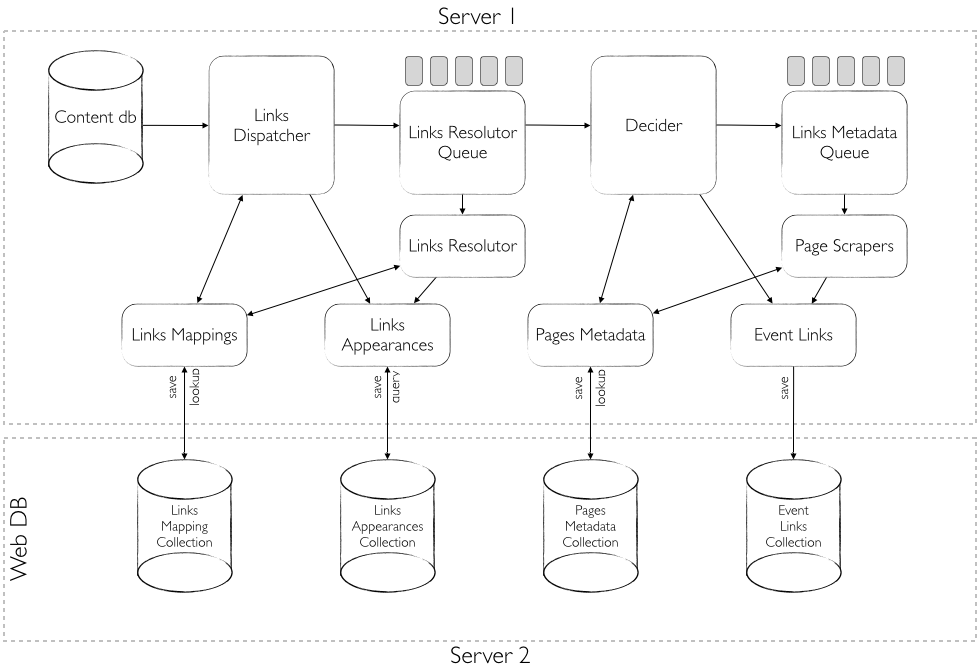
\includegraphics[width=8cm]{Figures/links_processing_architecture.png}
  \caption{Architecture of the system.}
  \label{fig:architecture}
\end{figure}

The complete processing for each link includes two very severe bottlenecks that require network calls that may take a couple of seconds to complete: the url resolution, and the page scraping. In order to overcome this limitation and build a more efficient system, we split the processing to two systems, intended to run in parallel.

The first issue addressed by the system is the fact that, due to URL shorteners and non-canonical URL formats, links to the same resources (e.g. http://new.com/some\_article) can take different forms (e.g. a bit.ly link, a URL that includes with different query strings, etc.).  

The \emph{links dispatcher} is the first step of this processing chain. It retrieves from the \emph{content database} all the event tweets for a recent temporal window. After loading the raw data, the links dispatcher extracts every link from the tweets' entities (\cite{RestTweetsDoc}), and queries the \emph{links mappings} data to check if the URL has already been resolved to a canonical form. If the link was not yet resolved, the system adds the URL to a \emph{link resolutor queue}. If it was already resolved, the system adds the link, together with the data about the tweet, to the \emph{links appearances} database. 

The links resolutor queue is implemented as a jobs queue\cite{RedisQueues}. The advantages of a jobs queue approach is that many workers instances can be run at the same time, and their number and behavior can be adjusted according to the workload. This allows for great flexibility in the way the system can be scaled depending on the abundancy of data.
%THEY KNOW WHAT A QUEUE IS. This means that a list of pointers to python functions and their arguments is stored in a Redis database for later execution.  The processes responsible of reading job queues and executing them are called ``workers''. 
All the urls in the queue are resolved by the \emph{links resolutor} function. This function will first look the url up in the links mappings and, if it is not found, it resolves the url and eventually saves a new mapping. When a link is successfully resolved, it is added to the \emph{links appearances} and a new mapping is saved.

The \emph{links appearances} dataset is the collection of all the resolved links. Every item contains information about the url, the tweet that contained it and the event that the tweet and url were part of. %In fact, multiple items might carry data about the same combination of url and tweet as long as they reference different events.

Links appearances are periodically accessed by the \emph{decider}, which is responsible for ranking the resources and filtering them as needed. The computation is always done on a sliding temporal window of fixed size. The scoring system relies on \emph{links score processors} for its decision process: different score processors can be implemented for testing different score functions. We detail the links score processors (LSPs) used for our experiments in sections~\ref{sec:volume_based_links_selection} and~\ref{sec:velocity_based_links_selection}. The LSPs we use only implement a very basic first filtering: their main function in the experiments discussed in this paper consist in enriching the event links with features useful for ranking. More consistent filtering possibilities are provided by our front-end interface.\todo{Make sure we explain how}

If a link is selected for publication, the decider queries the \emph{pages metadata} database to check whether the system has the available metadata for that link. If no metadata is available, the link appearance is added to the \emph{Links Metadata Queue}, otherwise it is saved together with its metadata as an \emph{event link}. 

The \emph{Links Metadata Queue} is processed by the \emph{metadata scraper}. This function extracts the domain from the url and selects a scraper class accordingly, it loads the referenced page and extracts pieces of information from it (e.g. a title, a description and a representative image). Different scrapers look for different tags in the DOM structure, as different websites usually expose different information in different ways. In our tests, we use a generic scraper that collects information stored in Open Graph and Twitter Cards meta-tags. Only links for which enough metadata is found are saved as event links, and pages metadata database is updated accordingly. % Ignore dups, for all they know we could be avoiding them altogether. If duplicate... duplicates are  while their scores and other relevant features are updated to the latest result.

The final output of the system is stored in the \emph{event links} database. This dataset holds the final set of resources, together with their score, and other attributes infered by the link score processor and used to rank the resource (e.g. total volume, highest volume in a time-window duration etc.). In addition, the record contains the metadata extracted from the referenced page\todo{ASSUMING ONE EVENT and the id of the event for which that link was processed. In fact, the same link can appear multiple times as long as it referenced different events.}

\section{Ranking Methods}
\label{sec:ranking_methods}
\todo{Write the sentence:}In this section, two methods of ranking...
\todo{Write me better:} Goals of ranking: 1) as early as possible and 2) robust: relevant and important. Not just every link -- not even all relevant links (may be too much). However, when something is relevant and important, identify it as early as possible. These are competing requirements, and we start with two very simple methods to see how they produce different results accprding to these requiremnts.


\subsection{Volume based LSP}
\label{sec:volume_based_links_selection}
\todo{Edit this para to say explicitly: the benefits of this method [links that are robust]. Drawbacks are [no emerging links, takes more time to be sure about any]}
Organizing a collection of every single appearance of every link gives us the possibility to obtain information about the volume of shares reached by a link during the event. As an example, Figure \ref{fig:batkid_whitehouse_volume} shows the number of appearances in time of the link to president Obama's Vine for Batkid\footnote{An initiative of Make-A-Wish Foundation for a child affected by leukemia and that attracted the attention of social media: http://abcnews.go.com/US/batkids-make-transforming-san-francisco-gotham/story?id=20899254; President Obama posted a Vine response at LINK TO VINE}.
\begin{figure}[htbp]
  \centering
  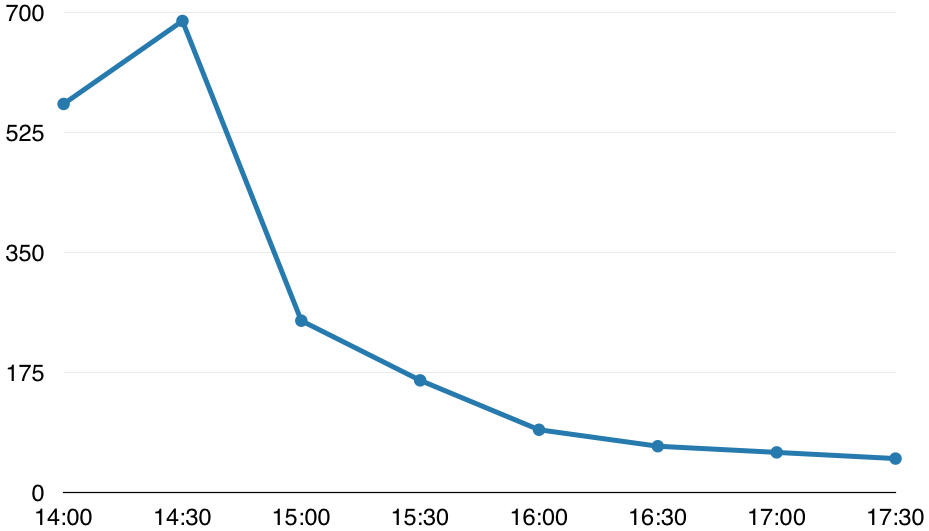
\includegraphics[width=\linewidth]{Figures/batkid_whitehouse_volume.png}
  \caption{Volume of president Obama's Vine video for Batkid shares.}
  \label{fig:batkid_whitehouse_volume}
\end{figure} \todo{Higher time-resolution excel graph}

The volume based LSP assigns to every link a score equal to the cumulative function of its volume throughout the event. A very basic filtering step is implemented by a manually chosen volume threshold that is only meant to exclude the noise of links that did not trigger any interest at all in the audience, and can be considered to be background noise (e.g. those links with only one appearance). Such threshold should be set according to the general volume of an event: we euristically tune these thresholds after extracting from the database aggregated statistics regarding the volume of these links. 

A link that has been shared at a nearly constant rate during the analyzed time range will be more likely to appear in our timeline than a link that reached a very high volume at a particular point in time. The display time for links ranked by this LSP is choosen to be the time of the earliest appearance that passed the elementary filtering (e.g. the second appearance of a link). Even if the precision of this parameter will suffer from setting very selective volume filters, we are assuming that high-volume events imply a faster growth of the volume of relevant links, thus introducing only smaller delays.

\subsection{Velocity based LSP}
\label{sec:velocity_based_links_selection}
\todo{Say explictiy: the benefits of this method; the drawbacks (more noisy).}
The velocity based LSP computes links' scores as the appearances volume reached by a link within one decider processing time window. The decider's time windows occur every 20 minutes and are 30 minutes long, thus allowing a 10 minutes overlap between each window.

This LSP implements the same filter described in Section \ref{sec:volume_based_links_selection}, with the only difference that the threshold is compared with the current time window's volume. The display time is defined as the first time a link appearance survives the filtering for the first time in a time window. However, the score is always updated to the highest volume the link has reached within a window.

\section{Front-end Interface}
\todo{Write out: In this section, we discuss sample presentation for extracted resources... only one way to expose these links, useful for this paper}

The results of the resource extraction process can be displayed in a simple interface, forming a ``storyline'': the list of resources are sorted chronologically according to a \emph{display time} field defined by the LSP. A filtering functionality can allow a user to select a cutoff score for the links to be visualized. When clicking on a link, that link is marked as false-positive. This marking functionality is used to plot the number of links satisfying a certain volume threshold versus the true-positives satisfiyng the same requirements. This interface also draws a pie chart, representing the source domains of the links displayed (taking into account the filtering parameter).

Figure \ref{fig:javascript_interface} shows a simple example of the storyline. The attributes shown for every link must be interpreted according to the LSP that produced them, this will be explained after introducing each LSP. This example uses the information scraped for each resource to create a visual representation of the contents, and an ``information scent'' for users to decide whether they'd want to click through. %Moreover, the combination of an image and a description for each resource can offer a more complete information than a tweet alone.
\begin{figure}[htbp]
  \centering
  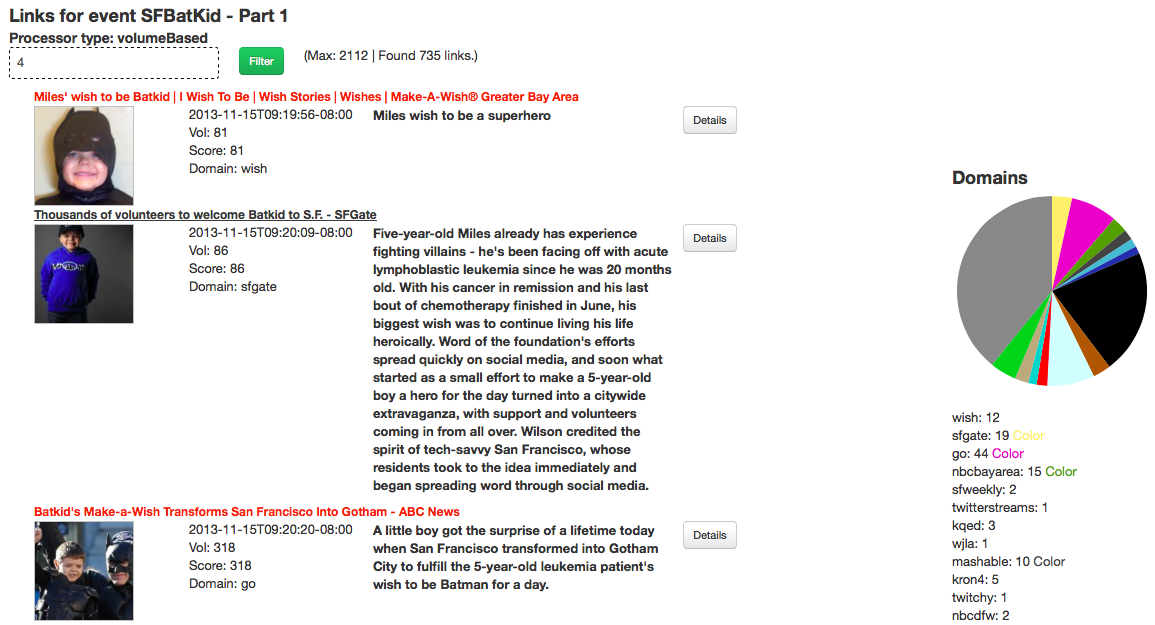
\includegraphics[width=8cm]{Figures/javascript_interface.png}
  \caption{Front-end interface easing the process of extracting and visualizing data.}
  \label{fig:javascript_interface}
\end{figure}

%%%%%%%%%%%%%%%%%%%%%%%%
%%%  4. Experiments  %%%
%%%%%%%%%%%%%%%%%%%%%%%%

\section{Experiments}
\label{sec:experiment}
In this section we describe the experiments made to evaluate the efficacy of the storylines built using our method, and to compare the results obtained with different LSPs. We choosed three events that feature very diverse characteristics:
\begin{description}
\item[Kanye West at Barclays Center] A concert of the ``Resurrects Yeezus'' tour, that took place in the very young New York venue. This event has a relatively low volume of 794 links shared on Twitter during 5 hours. We will refer to it as ``\#kenye''.
\item[Tech Crunch Disrupt] The 2013 conference held in San Francisco. This is a longer event that lasted 3 days (80 hours of content gathered) with a total links volume of 1201. We will refer to this event as ``\#TCDisrupt''.
\item[San Francisco's Batkid] An event organized by the Make a Wish Foundation, that transformed San Francisco in Gotham City for one day, letting a child affected by leuchemia help Batman to fight the chrime. This is a very high volume event, with 8842 links shared, during a timespan of 9 hours. When mentioning this event in the following sections, we will use its hashtag: ``\#SFBatkid''.
\end{description}

Every event has been processed with both the LSPs presented in Section \ref{sec:ranking_methods} using the minimum threshold possible: 1 for \#Kanye and \#TCDisrupt, while a threshold of 4 has been used for \#SFBatkid in order to obtain a number of links that could be handled by the javascript interface. For \#SFBatkid, we extracted the data regarding lower thresholds by directly querying the database.

When collecting data to compare the number of true-positives against the number of false-positives, we first filtered the displayed links according to a volume threshold high enough to only select less than 100 links (number that we considered to be optimal for obtaining an enjoyable storyline), and then we proceeded with the false-positives marking process.

During our experiments, we also monitored the composition of the domains generating all the links, and the way they varied according to different filter settings. This approach, surfaced interesting information that could help automatically improve the quality of these storylines.

In Section \ref{sec:dataset} we clarify what system constitutes the data source for our experiments, as well as how data is stored in such system. We then comment the quality and characteristics of the storylines obtained for each event in section \ref{sec:storylines}. In sections 

\subsection{Notes and ideas to write about experimental results.}
\begin{itemize}
\item Events chose to represent low/medium/high volume events and three different categories (conference,music,breaking news), they are past events, but the processing simulates the same mechanism that acts on happening events.
\item Sources pies
  \begin{itemize}
    \item Highlighted are every time those sources that had more relevance in the particular event (there is no color for NBC news in the TechCrunch event)
    \item Results distorted by broken links and because of Twitter's audience and usage.
    \item Filter steps choosen to better show how the sources composition changes according to the volume requested. Usually, it's more interesting what happens for volumes 1,2,3, as higher numbers don't reveal a statistic anymore, and are distorted by outliers.
  \end{itemize}
\item Volume/Cardinality graph
\begin{itemize}
    \item Green line: true positives, blue line: total
    \item A filter threshold is selected so that a more readable number of items is visible (less than 100).
    \item After filtering by such threshold, false positives that are still visible are selected (This is why plots don't show the true-positives curves for the first values of the series).
    \item Those items that are completely unrelated to the event, and those items that are related to the topic of the event but not to the event itself, are marked as false positives.
    \item ALSO REMOVED CONTENTS (e.g. Instagram pages saying the photo does not exist) are considered false positives.
\end{itemize}
\end{itemize}

\subsection{Dataset}
\label{sec:dataset}
The data used in our experiments is provided by Seen\footnote{http://seen.co}, a service offered by Mahaya, Inc. that aims at organizing social media by building automatic summaries of events \cite{SeenWired}. An event can be defined on this system by specifying a set of hashtags and a time range. Once these parameters are known, the contents database (shown in Figure \ref{fig:architecture}) is constantly updated with new raw data gathered from different social platforms at regular intervals in time, until the end of the event.

Events' metadata is saved to a collection in a different database (the web database of Figure \ref{fig:architecture}). Initially, metadata only comprehends parameters specified by the user, but it is later enriched with meaningful information utomatically inferred by the service. For our software, only the metadata specified by the user is needed to retrieve the right subset of raw contents from the contents database. However we only select events that already exist on the platform, so that we can first acknowledge the general characteristics of each of them in terms of data flow.

\subsection{Storylines}
\label{sec:storylines}
\subsubsection{Kanye West at Barclays Center}
The storyline obtained for this low volume event is very close to what we would expect from a low volume music event. In fact, data appears to be noisier, as many links are more generally related to the artist. Some examples are links to his music video that apparently came out in the same period when the concert took place, and links his tracks on the iTunes Store. This problem affects the timeline until around 8PM. At that point the concert must have effectively started, because between 8PM and 23PM the storyline is only populated by Instagrams depicting various moments of the performance. This strongly visual component is another characteristic that probably characterizes most performance-related events.

\subsubsection{Tech Crunch Disrupt}
The links telling the story of the \#TCDisrupt conference are particularly efficient in describing what happened at different detail levels. They are almost uniquely news articles, thus accompanied by incredibly descriptive images, titles and descriptions. The first day of conference contains most of the links, because it includes a number of general references to the conference itself and to the hype for its beginning. However the time references seem to be correct: the first item is actually about the first application that was pitched, and according to some following resources this project caused a sexist scandal, followed by Tech Crunch's official excuses.

Further down in the timeline, the links/day ratio shrinks, and increases its quality as it mostly includes specific articles about the presentations held on days two and three in chronological order. In particular, the last item closes the storyline by declaring the winner of \#TCDisrupt.

\subsubsection{San Francisco's Batkid}
This event, under the social point of view, has a very particular configuration: it consists of huge amounts of content (tens of thousands of tweets) shared in a relatively limited amont of time, mostly as the echo of mass-medias' voice. The resulting narration, when filtered down to a human readable length of 100 items, is very general and redundant, mostly composed by articles that describe the event as a whole. Instant media (for example, Instagrams) has been drowned by the huge numbers of shares achieved by sources like CNN and NBC. As a result, this timeline is almost exempt from noise but it is very inefficient at narrating the event.

\subsection{Selection and Ranking quality of Different LSPs}
\label{sec:selection_and_ranking_quality}
We filtered the storylines resulting from the velocity and volume based processors until we obtained less than 100 items, then we marked the false-positive results and we plotted the number of results and the number of true-positives obtained with increasing thresholds. The first important difference we noticed between the two LSPs is the quality of the ranking: while the velocity based LSP tends to concentrate most of the results in the left-most part of the plot (thus in the lower part of the ranking), the volume based one distributes the results better. This strong difference can be seen in Figure \ref{fig:tcdisrupt_plots}.
\begin{figure}[htbp]
  \centering
  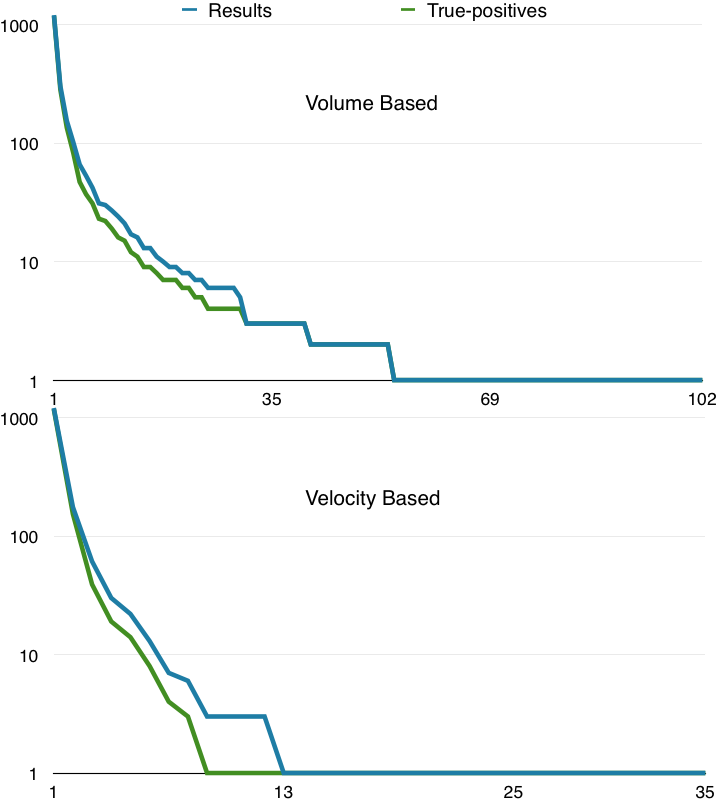
\includegraphics[width=8cm]{Figures/tcdisrupt_plots.png}
  \caption{Number of results and number of true-positive resultsfor increasingly higher riltering thresholds obtained thanks to the volume based LSP and the velocity based LSP for the TCDisrupt event.. }
  \label{fig:tcdisrupt_plots}
\end{figure}

Figure \ref{fig:tcdisrupt_plots} also indicates a substantial efficacy in selecting true-positive results when filtering the output of the volume based LSP. This was not observed with the other two events, where the performance difference between the two LSPs under this point of view was irrelevant undistinguishable.

A characteristic of the plot made on velocity based results is the way there usually are a very limited number of highly referenced links that are underlined by their distance from lower-ranked resources. This can be seen in Figure \ref{fig:tcdisrupt_plots} as well as in Figure \ref{fig:sfbatkid_plot}, where the top ranked item is a Vine of president Barak Obama congratulating with the young superhero. Although, those few outliers with very high values, happened to be, in all our experiments, true positives (they could used as ``highlighted'' links or reccomendations).
\begin{figure}[htbp]
  \centering
  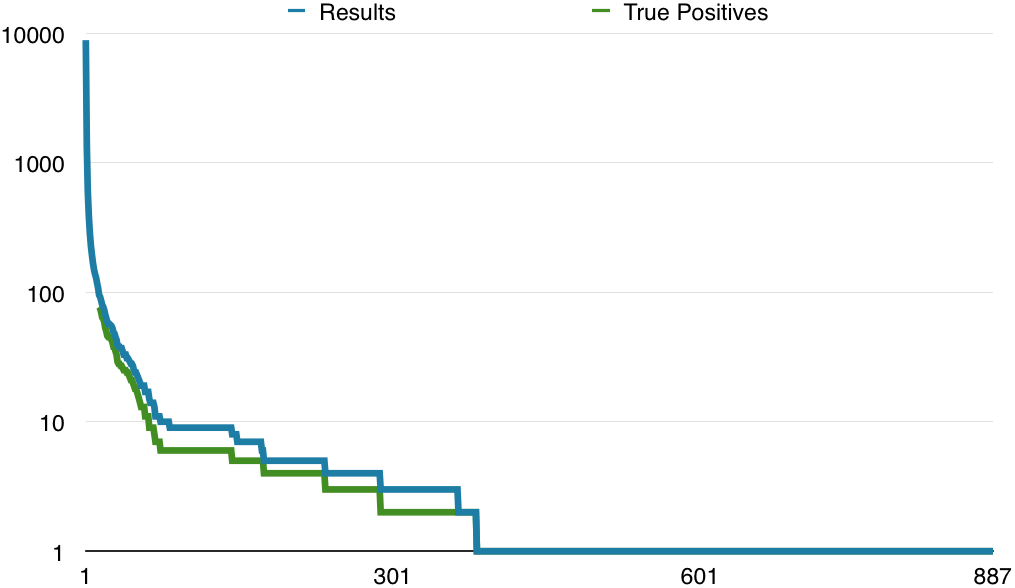
\includegraphics[width=8cm]{Figures/batkid_plot.png}
  \caption{Number of results and number of true-positive resultsfor increasingly higher riltering thresholds obtained thanks to the velocity based LSP for the SFBatkid event.}
  \label{fig:sfbatkid_plot}
\end{figure}
This same characteristic is common to all the top ranked elements obtained with the velocity-based method, thus making this selection system reliable for choosing elements to recommend as interesting higlights.

\subsection{Domains Composition}
\label{sec:domains_composition}
The analysis of the source domains underlined how different categories of events can have a very different ``fingerprint'' in this space. Figure \ref{fig:category_domains} clearly shows how a performance-centered event mostly received data from Instagram and Youtube, while a breaking news event and a technological conference are described by a wider variety of newspapers and magazines operating in the respective fields.
\begin{figure}[htbp]
  \centering
  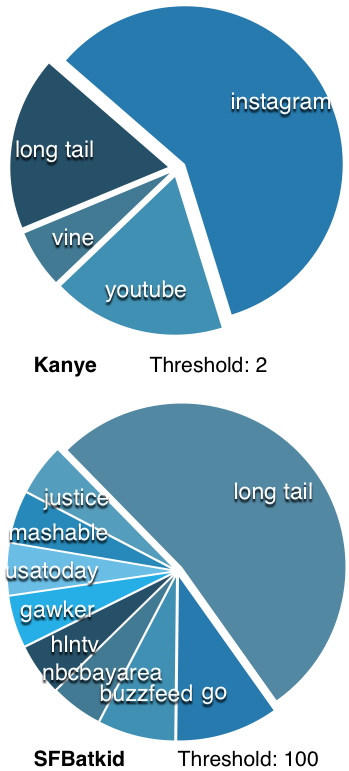
\includegraphics[width=5cm]{Figures/category_domains.png}
  \caption{Source domains composition for the SFBatkid and the Kanye events. Volume thresholds have been chosed as the highest that still allowed enough results to produce a meaningful analysis.}
  \label{fig:category_domains}
\end{figure}
This information could be used to automatically detect events' categories, or to implement a smarter ranking function thath assigns different importance to links coming from different sources, when the category of the event is known. We also noticed how some of the biggest generators of social content (i.e. Instagram, Facebook) tend to disappear from the pie chart when rising the volume threshold above one. This underlines the importance of a third dimension, the volume, in defining a ``category fingerprint'' in this particular space of the source domains.

This analysis space can also help to automatically identify official sources for a given event. In fact, if the category fingerprint of an event is given, official sources can sometimes be identified as outliers: this can be clearly seen in figure \ref{fig:tcdisrupt_outlier}, where the ``techcrunch'' domain has a clearly outsized cardinality comparing with the other sources.
\begin{figure}[htbp]
  \centering
  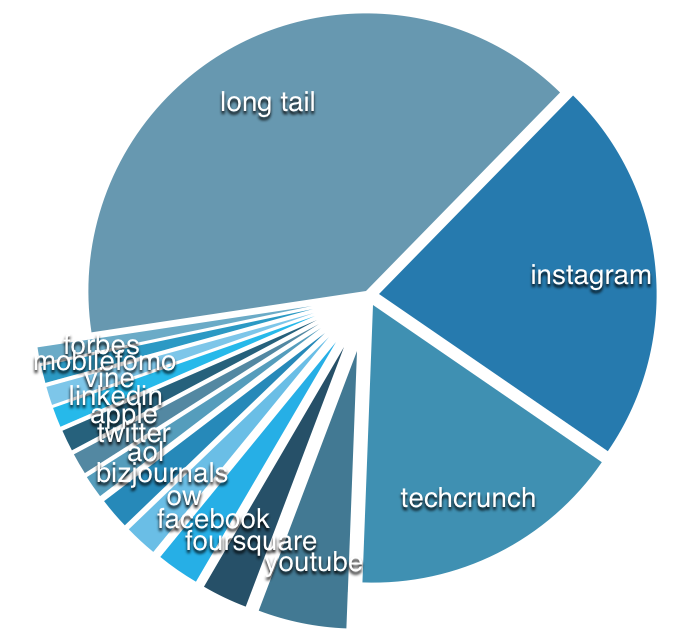
\includegraphics[width=5cm]{Figures/tcdisrupt_outlier.png}
  \caption{Source domains of the TCDisrupt event, computed on results obtained without any filtering.}
  \label{fig:tcdisrupt_outlier}
\end{figure}
%%%%%%%%%%%%%%%%%%%%%%%%%%%%%%%%%%%%%%%
%%%  6. Conclusion and Future Work  %%%
%%%%%%%%%%%%%%%%%%%%%%%%%%%%%%%%%%%%%%%

\section{Conclusion and Future Work}
\label{sec:conclusions}
\todo{better Deduplication,.}

\section{Acknowledgments}
\label{sec:ack}

\nocite{*}
\bibliographystyle{abbrv}
\bibliography{seen}
\balancecolumns
% That's all folks!
\end{document} 
